% !TeX root = RJwrapper.tex
\title{\pkg{shinybrms}: Fitting Bayesian Regression Models Using a Graphical User Interface for the R Package \pkg{brms}}
\author{by Frank Weber, Katja Ickstadt, and \"Anne Glass}

\maketitle

\abstract{
  Despite their advantages, the application of Bayesian regression models is
  still the exception compared to frequentist regression models. Here, we
  present our R package \CRANpkg{shinybrms} which provides a graphical user
  interface for fitting Bayesian regression models, with the frontend
  consisting of a \CRANpkg{shiny} app and the backend relying on the R package
  \CRANpkg{brms} which in turn relies on Stan. With \pkg{shinybrms}, we hope
  that Bayesian regression models (and regression models in general) will
  become more popular in applied research, data analyses, and teaching. Here, we
  illustrate our graphical user interface by the help of an example from medical
  research.
}

%%% USE THIS(?):
%\Keywords{Bayesian, regression model, graphical user interface, GUI, R, \pkg{shiny}, \pkg{brms}, Stan}
%%%

%%%%%%%%%%%%%%%%%%%%%%%%%%%%%%%%%%%%
\section{Introduction}
\label{intro}

The relevance of regression models in applied research has already been well
pointed out, for example, by \citet{karabatsos_menu-driven_2015}:
\begin{quote}
  ``Regression modeling is ubiquitous in empirical areas of scientific
  research. This is because most research questions can be asked in terms of
  how a dependent variable changes as a function of one or more covariates
  (predictors).''
\end{quote}

Conducting regression analyses in a \dfn{Bayesian} framework has a lot of
advantages. Introductory texts on Bayesian statistics (in general) are,
e.g., \citet{mcelreath_statistical_2020}, \citet{albert_probability_2019},
\citet{reich_bayesian_2019}, \citet{statacorp_introduction_2019},
\citet{gelman_regression_2020}, and \citet{johnson_bayes_2022}.
For readers with little background in Bayesian statistics, we recommend
reading one of these textbooks first. A more detailed introduction
may be found, e.g., in \citet{gelman_bayesian_2014}. In particular, Bayesian
statistics has the following advantages \citep[for further advantages, see,
e.g.,][]{gelman_bayesian_2014, statacorp_introduction_2019}:
\begin{enumerate}
  \item Bayesian methods allow for incorporation of \dfn{prior knowledge}.
  Generally, inclusion of prior knowledge is desirable: The flat prior implied
  by the frequentist maximum likelihood (ML) method may lead to nonsensical
  inferences \citep{gelman_prior_2017}. Even if the inclusion of informative
  prior knowledge is not desired, weakly informative priors have the advantage
  (compared to so-called ``noninformative'' priors\footnote{We added quotation
  marks here since noninformative priors might be more informative than intended
  \citep{gelman_prior_2017}.}) to downweight unreasonable parameter values and to
  introduce a certain \dfn{regularization} or \dfn{penalization}, helping against
  overfitting \citep{gelman_prior_2006, gelman_weakly_2008, gelman_bayesian_2014,
  gelman_prior_2017}. Hereafter, we follow conventional notation in Bayesian
  statistics and denote the prior for the parameter vector $\boldsymbol{\theta}$
  by $p(\boldsymbol{\theta})$.

  \item Similarly, the prior distribution may be used to impose \dfn{parameter
  constraints} in an easy and natural way. There is no need for \textit{ad-hoc}
  solutions to cut off parameter estimates. For example, many frequentist
  between-study variance estimators in the random-effects meta-analysis model
  are cut off at zero.

  \item It is usually possible to infer the posterior \dfn{exactly} (apart from
  minor approximations such as those arising from the Monte Carlo error). In
  that case, Bayesian statistics does not need to resort to large-sample
  approximations such as the asymptotic normal distribution of the ML estimator
  often used in frequentist statistics.
  
  \item For most practical cases, Markov chain Monte Carlo (MCMC) sampling (see
  section~\nameref{algos-mcmc}) constitutes a \dfn{generic} Bayesian inference
  method. In frequentist statistics, generic methods such as the asymptotic
  normal distribution of the ML estimator can be unsatisfactory, e.g., for
  small sample sizes. This is why in frequentist statistics, different
  inferential methods have often evolved for the same task or model. This
  complicates frequentist analyses for users, especially for those with
  little background in statistics.

  \item The quantities derived from the posterior have a \dfn{more intuitive
  interpretation} than their frequentist counterparts which are based on the
  sampling distribution of the estimator. In particular, Bayesian posterior
  intervals (credible intervals, CrIs) have the interpretation that is often
  incorrectly attributed to frequentist confidence intervals (CIs)
  \citep{mcelreath_statistical_2020} and posterior tail-area probabilities
  have the interpretation that is often incorrectly attributed to frequentist
  $p$-values.

  \item In Bayesian statistics, \dfn{uncertainty in nuisance parameters} is
  easily---and naturally---taken into account by integrating them out from
  the posterior:
  \begin{equation}
  p(\boldsymbol{\psi} | \boldsymbol{\mathcal{D}}) =
  \int p(\boldsymbol{\psi}, \boldsymbol{\phi} | \boldsymbol{\mathcal{D}})
  \; \text{d}\boldsymbol{\phi}
    \label{eqn:nuisance}
  \end{equation}
  with $\boldsymbol{\mathcal{D}}$ denoting the data, $\boldsymbol{\psi}$
  the parameter vector of interest, and $\boldsymbol{\phi}$ the nuisance parameter vector (so that
  $(\boldsymbol{\psi}^\tp, \boldsymbol{\phi}^\tp)^\tp = \boldsymbol{\theta}$)\footnote{Here, we are
  slightly abusing the notation by employing a single integral symbol for a possibly multiple integral.}.
  Taking uncertainty in nuisance parameters into account helps against overfitting
  (like the penalization mentioned in enumeration point number~1 above), but
  in general, this is not that easy in frequentist statistics, as can be seen in
  random-effects meta-analyses \citep{weber_interval_2021}.

  \item When combined with probabilistic programming (as done, e.g., by the
  various sampling methods introduced in section~\nameref{algos}), a Bayesian
  analysis naturally \dfn{propagates the posterior uncertainty} into derived
  quantities \citep{gelman_regression_2020}.

  \item Often, frequentist analyses result in the typical \dfn{null-hypothesis
  significance testing} which is being criticized to an increasing degree
  \citep{amrhein_remove_2018, amrhein_scientists_2019,
  mcshane_abandon_2019}. Null-hypothesis significance testing is especially
  problematic for null hypotheses consisting of only a point in parameter
  space. Of course, Bayesian analyses may also result in null-hypothesis
  significance testing or similar hypothesis-testing procedures, but in our
  experience, this is not as common as in frequentist analyses. We designed our
  software presented here in a way that does not encourage null-hypothesis
  significance testing.

  \item \dfn{Posterior predictive checks (PPCs)}---which should be part of a
  Bayesian workflow \citep{gelman_bayesian_2020}---are an easy and intuitive
  way of performing model diagnostics in a Bayesian framework, even though the
  choice and interpretation of the PPCs require some experience
  \citep{gelman_bayesian_2020}. In a frequentist framework, model
  diagnostics are often not that easy to perform, at least if the uncertainty
  from parameter estimation should be taken into account.
\end{enumerate}

These advantages will be illustrated in the context of the example from
section~\nameref{exmpl}, by comparing our Bayesian analysis to a frequentist
one (see section ``Frequentist analysis of the example'' in the online
Supplement file \file{Supplement\_sections.pdf}).

Despite the aforementioned advantages, Bayesian methods---and Bayesian
regression models (BRMs) in particular---are still not as common as their
frequentist counterparts. In 2005, \citet{woodward_bugsxla_2005} supposed one
reason to be the lack of a ``good user interface'' which would allow
applied researchers to fit BRMs as conveniently as other statistical methods
for which a graphical user interface~(GUI) already exists. In the meantime,
several GUIs have emerged (see section~\nameref{GUIs}), but to our knowledge,
until the first release of our R package
\pkg{shinybrms} \citep{weber_shinybrms_2021}, there was no GUI which used
Stan \citep{carpenter_stan:_2017, stan_development_team_stan_2022} for
inferring the posterior in BRMs. Stan has several advantages compared to other
methods for inferring the posterior. In particular, it is highly flexible with
respect to modeling choices and very efficient. Details will be given in
section~\nameref{algos}.

Our \pkg{shinybrms} package is noncommercial and available at the
Comprehensive R Archive Network~(CRAN). While \pkg{shinybrms}'s frontend
is a \pkg{shiny} \citep{chang_shiny_2021} app, \pkg{shinybrms}'s backend
completely relies on \pkg{brms} \citep{burkner_brms:_2017,
burkner_advanced_2018} which itself relies on Stan. Both of \pkg{brms}'s
backends (i.e., interfaces to Stan), namely \CRANpkg{rstan}
\citep{stan_development_team_rstan_2020} and \pkg{cmdstanr}
\citep{gabry_cmdstanr_2020}, are supported by \pkg{shinybrms}. For the
inspection of the Stan output, the \CRANpkg{shinystan}
\citep{gabry_shinystan_2018} app may be launched from within \pkg{shinybrms}.

To explain the particular advantages of Stan in detail, we have to take a closer
look at different ways for inferring the posterior. This is the purpose of
section~\nameref{algos}. In section~\nameref{GUIs}, we summarize existing GUIs for
BRMs. That section is partly influenced by \citet{ramirez-hassan_guided_2021}.
In section~\nameref{feat}, we present the features of \pkg{shinybrms}. The
usage of the \pkg{shinybrms} app is illustrated by the help of a real-world
example in section~\nameref{exmpl}. Finally, we discuss our work in
section~\nameref{disc}.

%%%%%%%%%%%%%%%%%%%%%%%%%%%%%%%%%%%%
\section{Algorithms for inferring the posterior}
\label{algos}

As mentioned above, in Bayesian statistics, uncertainty arising from the
estimation of nuisance parameters is taken into account by integrating them
out from the posterior. This is not the only integration occurring in
posterior inference: Basically every quantity derived from the posterior is
somehow connected to an integration over the posterior. However, it is the
integration which also causes a lot of complications. While it is most
desirable to perform posterior inference by exact calculation of the desired
integrals (using analytic expressions), this approach is often infeasible and
even if it is feasible, it has the downside of being not as flexible as other
approaches since it needs to be tailored to the statistical model at hand.
Numerical integration (e.g., by quadrature) may seem like a remedy, but is
often only feasible up to a limited dimensionality of the parameter space.
Depending on the algorithm, numerical integration may also introduce tuning
quantities, hindering its ``out-of-the-box'' usage.
Integration by simple Monte Carlo (MC) sampling may seem like an alternative,
but this is only possible for distributions one may directly sample from
(e.g., a Gaussian distribution).

%%%%%%%%%%%%%%%%%%
\subsection{Markov chain Monte Carlo}
\label{algos-mcmc}

With the advent of Markov chain Monte Carlo (MCMC) methods, Bayesian inference
has changed a lot \citep{woodward_bugsxla_2005, lunn_bugs_2009}. The first
MCMC algorithm was the \dfn{Metropolis} algorithm
\citep{metropolis_equation_1953} which starts from an initial point in
parameter space and iteratively samples a \dfn{proposal}\footnote{Here,
the term ``proposal'' refers to a proposed parameter vector.} from a
\dfn{symmetric}\footnote{Here, the term ``symmetric'' refers to the preservation
of the distribution when reverting the jump, not to the symmetry in the shape of
a distribution.} jumping distribution and accepts the proposal with a certain
acceptance probability which depends on the ratio of the target (here, the
posterior) density at the current position and at the proposal. The
\dfn{Metropolis-Hastings (MH)} algorithm \citep{metropolis_equation_1953,
hastings_monte_1970} generalizes the Metropolis algorithm to asymmetric
jumping distributions. \dfn{Gibbs sampling} \citep{geman_stochastic_1984,
gelfand_sampling-based_1990} consists of alternately sampling from the full
conditional posterior distributions and is a special MH algorithm in which the
proposal is always accepted \citep{gelman_bayesian_2014}. Combinations of
the aforementioned algorithms are also widely used, e.g., MH-within-Gibbs.
All MCMC algorithms (including those mentioned hereafter) require a careful
examination of the convergence of the Markov chains. The MCMC diagnostics used
for this purpose in \pkg{shinybrms} are outlined in section~\nameref{tab-MCMC}.

\dfn{Hamiltonian Monte Carlo (HMC)}
\citep[initial work and major contributions by][]{duane_hybrid_1987,
neal_probabilistic_1993, mackay_information_2003, neal_mcmc_2011} is a special
MCMC algorithm which is
often more efficient than other MCMC algorithms, especially in case of a
high-dimensional posterior distribution and correlated parameters
\citep{hoffman_no-u-turn_2014, betancourt_conceptual_2018}. The efficiency
of HMC is due to the fact that it takes advantage of the gradient of the (log)
posterior density \citep{stan_development_team_reference_2022}, making it a
combination of stochastic and deterministic procedures (which explains why HMC
is also known as \dfn{hybrid Monte Carlo})
\citep{gelman_bayesian_2014}. HMC provides helpful diagnostics, such
as divergent transitions which can (but must not necessarily) indicate areas
of the posterior which are hard to explore by the HMC sampler
\citep{betancourt_conceptual_2018, gabry_visualization_2019}. Compared to
Gibbs sampling, HMC also has the advantage that nonconjugate priors may be
used easily. For the original HMC algorithm, three tuning quantities need to
be specified by hand in advance: the \dfn{mass matrix}~$\boldsymbol{M}$ (which
is the covariance matrix of the auxiliary momentum vector), the number~$L$ of
\dfn{leapfrog steps}, and the size~$\epsilon$ of the leapfrog steps
\citep{gelman_bayesian_2014, stan_development_team_reference_2022}.

Because of the fixed choice of~$L$, the original HMC algorithm is a
\dfn{static} HMC algorithm \citep{betancourt_conceptual_2018}. In
contrast, the \dfn{no-U-turn sampler (NUTS)}
\citep{hoffman_no-u-turn_2014} is a \dfn{dynamic} HMC algorithm since it
automatically chooses a (possibly) new value of~$L$ in each iteration of each
Markov chain. \citet{hoffman_no-u-turn_2014} also proposed a new dual
averaging technique for determining~$\epsilon$ automatically, too. Apart from
these automations, the NUTS has the advantage that in terms of efficiency, it
was shown to perform as well as---or even better than---a well-tuned static
HMC algorithm \citep{hoffman_no-u-turn_2014}. A modified
\citep{betancourt_conceptual_2018} NUTS
is implemented in Stan. Stan's
NUTS also includes an automatic adaptation of the mass matrix~$\boldsymbol{M}$
during the warmup phase \citep{stan_development_team_reference_2022}. A complete
presentation of Stan's NUTS is out of the scope of this article. A good
starting point for a detailed description is
\citet{stan_development_team_reference_2022} as well as
\citet{betancourt_conceptual_2018}. Note that Stan also includes other
algorithms for inferring or approximating the posterior. In this paper
however, we only refer to Stan's NUTS when referring to Stan.

%%%%%%%%%%%%%%%%%%%%%%%%%%%%%%%%%%%%
\section{Existing GUIs}
\label{GUIs}

Table~\ref{tab:GUIs} summarizes existing GUIs for BRMs. Details are provided
in Supplement section ``Existing GUIs''.
Table~\ref{tab:GUIs} makes it clear that none of the existing GUIs relies
\emph{entirely} on Stan or the NUTS.
\begin{sidewaystable}[htpb]
  \centering
  \caption{Existing GUIs for BRMs. Algorithmic details for the GUIs may be found in Supplement section ``Existing GUIs''. ``BB'' stands for ``Bayesian bootstrap''. Here, the term ``NUTS'' includes Stan's NUTS. The column ``Algorithm choice'' specifies if given a model, the user may choose an algorithm (at least for some types of models). Notes: (i) The TEET package is noncommercial, but MATLAB is commercial; (ii) JASP uses (Stan's) NUTS for Bayesian meta-analyses and mixed BRMs; (iii) For linear regression models, BEsmarter offers a choice between MCMC and the Bayesian bootstrap.}
  \label{tab:GUIs}
  \begin{tabular}{ll|llll|lll|l}
    \toprule
    & & \multicolumn{7}{c|}{Algorithm (for inferring the posterior)} & \\
    & & \multicolumn{4}{c|}{Non-MCMC} & \multicolumn{3}{c|}{MCMC} & \\
    GUI name & Commercial & Analytic & Numerical & MC & BB & Non-HMC & Static HMC & NUTS & Algorithm choice \\
    \midrule
    WinBUGS \citep{lunn_winbugs_2000} & {\color{dgray}no} & {\color{dgray}no} & {\color{dgray}no} & {\color{dgray}no} & {\color{dgray}no} & yes & {\color{dgray}no} & {\color{dgray}no} & {\color{dgray}no} \\
    OpenBUGS \citep{spiegelhalter_openbugs_2014} & {\color{dgray}no} & {\color{dgray}no} & {\color{dgray}no} & {\color{dgray}no} & {\color{dgray}no} & yes & yes & {\color{dgray}no} & {\color{dgray}no} \\
    BugsXLA \citep{woodward_bayesian_2011} & {\color{dgray}no} & {\color{dgray}no} & {\color{dgray}no} & {\color{dgray}no} & {\color{dgray}no} & yes & yes & {\color{dgray}no} & {\color{dgray}no} \\
    IBM SPSS Amos \citep{arbuckle_amos_2020} & yes & {\color{dgray}no} & {\color{dgray}no} & {\color{dgray}no} & {\color{dgray}no} & yes & yes & {\color{dgray}no} & yes \\
    TEET \citep{qian_toolkit_2011} & {\color{dgray}no\textsuperscript{(i)}} & yes & yes & yes & {\color{dgray}no} & yes & {\color{dgray}no} & {\color{dgray}no} & {\color{dgray}no} \\
    JASP \citep{jasp_team_jasp_2020} & {\color{dgray}no} & yes & yes & yes & {\color{dgray}no} & yes & {\color{dgray}no} & yes\textsuperscript{(ii)} & {\color{dgray}no} \\
    BRNPM \citep{karabatsos_menu-driven_2015, karabatsos_menu-driven_2017} & {\color{dgray}no} & {\color{dgray}no} & {\color{dgray}no} & {\color{dgray}no} & {\color{dgray}no} & yes & {\color{dgray}no} & {\color{dgray}no} & {\color{dgray}no} \\
    Stata \citep{statacorp_stata_2019} & yes & {\color{dgray}no} & {\color{dgray}no} & {\color{dgray}no} & {\color{dgray}no} & yes & {\color{dgray}no} & {\color{dgray}no} & yes \\
    BayES \citep{emvalomatis_bayes_2020} & {\color{dgray}no} & {\color{dgray}no} & {\color{dgray}no} & {\color{dgray}no} & {\color{dgray}no} & yes & {\color{dgray}no} & {\color{dgray}no} & {\color{dgray}no} \\
    IBM SPSS \citep{ibm_corp_ibm_2020} & yes & yes & yes & yes & {\color{dgray}no} & {\color{dgray}no} & {\color{dgray}no} & {\color{dgray}no} & {\color{dgray}no} \\
    BEsmarter (\citealp{besmarter_team_besmarter_2020, besmarter_team_besmartergui_2020}; & {\color{dgray}no} & {\color{dgray}no} & {\color{dgray}no} & {\color{dgray}no} & yes & yes & {\color{dgray}no} & {\color{dgray}no} & yes\textsuperscript{(iii)} \\
    \citealp{ramirez-hassan_guided_2021}) & & & & & & & & & \\
    \bottomrule
  \end{tabular}
\end{sidewaystable}
JASP does use Stan for some analyses, but JASP's concept is
quite different from \pkg{shinybrms}'s concept: While JASP offers a
plenty of different statistical methods (including non-regression analyses),
\pkg{shinybrms} is designed to be as concise as possible. While JASP's
approach of using Stan for only some analyses
certainly has a few advantages (especially in terms of runtime),
\pkg{shinybrms}'s approach of completely relying on Stan (and \pkg{brms}
in particular) has the advantage of a better maintainability: \pkg{shinybrms}
only provides a lightweight GUI and only needs to perform few computations on
its own. This is due to \pkg{brms} which is very flexible by allowing to fit a
variety of regression models within a single R package. This division of
work between \pkg{shinybrms}, \pkg{shiny}, \pkg{brms}, \pkg{rstan}, Stan,
and \pkg{shinystan} reduces the amount of maintenance necessary for
\pkg{shinybrms}, resulting in a faster integration of new features, a faster
elimination of bugs, and a longer life cycle. Furthermore, it allows the
authors of each component to focus on their strengths.

%%%%%%%%%%%%%%%%%%%%%%%%%%%%%%%%%%%%
\section{Features of shinybrms}
\label{feat}

The following general presentation of \pkg{shinybrms}'s features will be in
written form, but with links to the corresponding screenshots from the example in
section~\nameref{exmpl}. In this article, not all aspects of the \pkg{shinybrms}
app are shown in screenshots. For more screenshots, see the \pkg{shinybrms}
website \citep{weber_shinybrms_2021}.

Note that the mathematical formulation of the models
which may be fit with \pkg{shinybrms} has already been given elsewhere
\citep{burkner_brms:_2017, burkner_advanced_2018}, so we will keep it short
here.

%%%%%%%%%%%%%%%%%%
\subsection{Overview}
\label{overview}

The \pkg{shinybrms} app has three main pages which are accessible from a
navigation bar at the top (Figure~\ref{fig:navbar-tree}):
``Likelihood'', ``Prior'', and ``Posterior''.
\begin{figure}[t!]
  \centering
  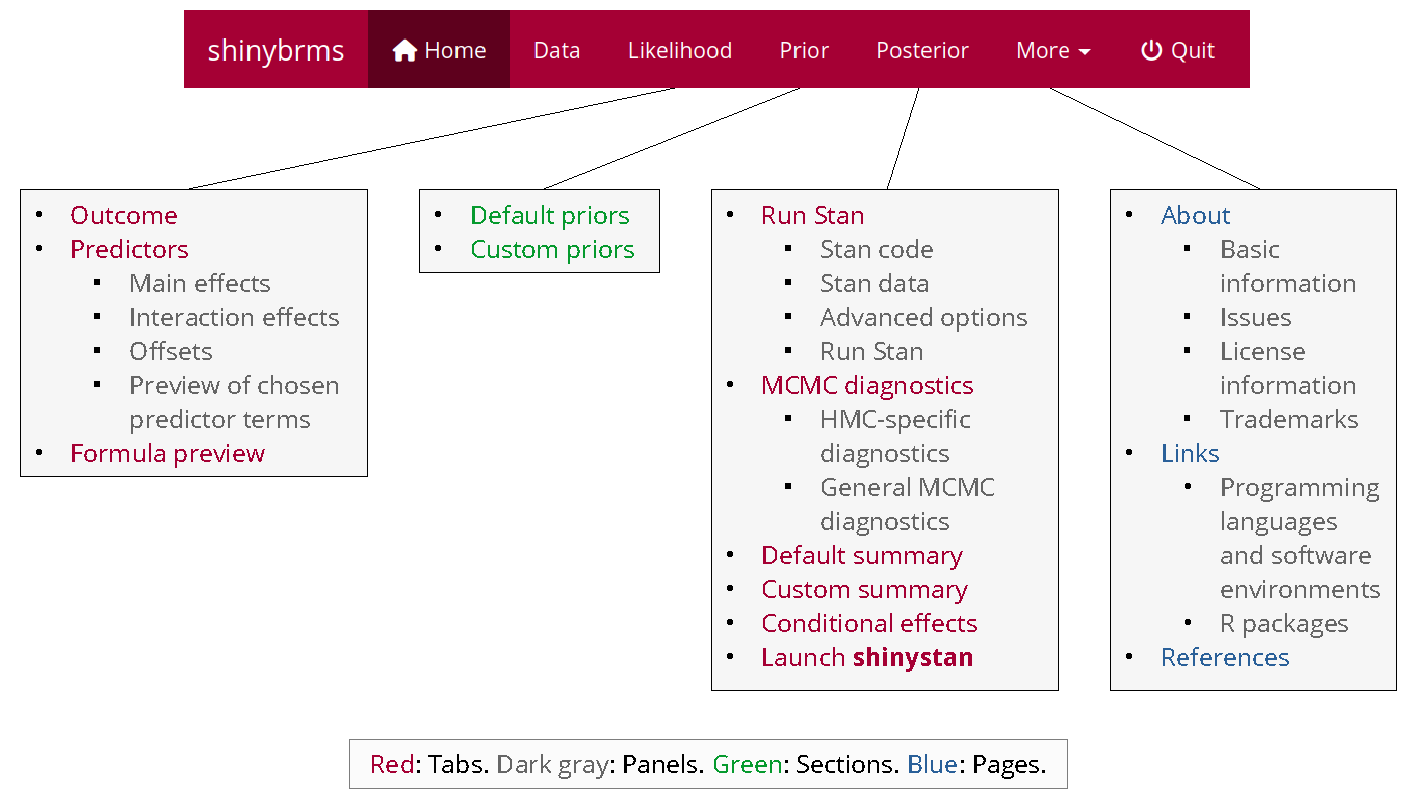
\includegraphics[width=\textwidth]{Figures/navbar_tree.pdf}
  \caption[Navigation bar]{The navigation bar in \pkg{shinybrms}.
  In this figure, we have expanded the navigation bar itself by the structure of the
  three main pages (``Likelihood'', ``Prior'', and ``Posterior'') as well as of the
  drop-down menu ``More''.}
  \label{fig:navbar-tree}
\end{figure}%
This structure follows Bayes' theorem, simplified to the proportionality of
the posterior density to the product of prior density and likelihood:
\begin{equation}
p(\boldsymbol{\theta} | \boldsymbol{\mathcal{D}}) \propto
p(\boldsymbol{\theta}) \cdot
p(\boldsymbol{\dot{\mathcal{D}}} | \boldsymbol{\theta}, \boldsymbol{\ddot{\mathcal{D}}})
  \label{eqn:bayes}
\end{equation}
where we have split up the data $\boldsymbol{\mathcal{D}}$ into
$\boldsymbol{\mathcal{D}} = \begin{bmatrix}\boldsymbol{\dot{\mathcal{D}}}
\;\; \boldsymbol{\ddot{\mathcal{D}}}\end{bmatrix}$
because in BRMs, the distribution in the likelihood typically conditions on the predictor
part~$\boldsymbol{\ddot{\mathcal{D}}}$ of the data (see section~\nameref{tab-pred} below).
In the following sections, these three main pages will be described in detail.

There are also some auxiliary pages, the first two having direct links in the
navigation bar, the last three being accessible from the drop-down menu ``More''
at the end of the navigation bar:
\begin{itemize}
  \item The starting page ``Home'' gives a short overview of
  \pkg{shinybrms}'s objective and structure. Thus, it only contains informational
  text and no interactive elements.

  \item On page ``Data'', the user uploads his or her custom dataset which shall
  be used for the regression analysis. For testing purposes, page ``Data'' also
  offers example datasets. The chosen dataset (no matter if it was uploaded or
  chosen from the list of example datasets) is automatically shown in a preview
  consisting of the dataset's first six rows (there is an option to show the
  full dataset, though). It is also possible to
  show the output of R's \code{str()} function applied to the chosen
  dataset, which gives some basic information about the dataset and its
  variables for users familiar with R.

  \item Page ``About'' contains basic information about \pkg{shinybrms}
  (e.g., version and corresponding date) as well as some legal information.

  \item Page ``Links'' gives links to software relevant for the
  \pkg{shinybrms} app.

  \item Page ``References'' contains the references for literature cited
  throughout the app.
\end{itemize}

%%%%%%%%%%%%%%%%%%
\subsection[Page "Likelihood"]{Page ``Likelihood''}
\label{page-lik}

Page ``Likelihood'' has three tabs: ``Outcome'',
``Predictors'', and ``Formula preview''. These tabs will now be
described in turn.

%%%%%%%%%
\subsubsection[Tab "Outcome"]{Tab ``Outcome''}
\label{tab-outc}

On tab ``Outcome'' (Figure~\ref{fig:outcome}), the user specifies the
outcome variable $\boldsymbol{y} = (y_1, \dotsc, y_N)^\tp \in \mathbb{R}^N$ (by
choosing it from a drop-down list of the variables present in the dataset) as
well as its distributional family, i.e., the basic form of the
likelihood~$p(\boldsymbol{\dot{\mathcal{D}}} | \boldsymbol{\theta}, \boldsymbol{\ddot{\mathcal{D}}})$,
now with $\boldsymbol{\dot{\mathcal{D}}} = \boldsymbol{y}$. For the distributional family, there is a
drop-down menu and a checkbox called ``Show advanced distributional families''.
By default, this checkbox is unchecked which means that the drop-down menu
offers three general distributional families of broad practical relevance:
the Gaussian family (with the identity link function), the Bernoulli family
with the logit link function, and the negative binomial family with the
log link function. This is intended to be a limited selection:
By reducing the choices as much as possible, we want to avoid
overwhelming the user with a variety of special distributions. For example,
the Poisson family is intentionally left out, in favor of the more general
negative binomial distribution. However, by checking the ``Show advanced
distributional families'' checkbox, the drop-down menu is extended so that
a variety of other distributional families can be selected as well (see
Supplement section ``Advanced distributional families'').

%%%%%%%%%
\subsubsection[Tab "Predictors"]{Tab ``Predictors''}
\label{tab-pred}

If desired, the user may specify predictors on tab ``Predictors''
(Figure~\ref{fig:predictors}). We use the term
``predictor'' for a column in the model matrix. In contrast, we use the
term ``predictor variable'' for a column in the input dataset. Thus, a
predictor may also denote an interaction and a predictor
variable with $K$ categories leads to $K - 1$ predictors (due to dummy
coding).

The \pkg{shinybrms} app supports population-level effects as well as
group-level effects\footnote{Population-level effects are also known as
fixed effects \citep{burkner_brms:_2017,
burkner_advanced_2018}. Group-level effects are also known as
random or partially pooled effects \citep{burkner_brms:_2017,
burkner_advanced_2018, goodrich_rstanarm_2022}. The terms ``fixed'' and ``random''
effects are not really appropriate in a Bayesian context: In a Bayesian model, all
parameters have a prior distribution and may therefore be considered as random
\citep{marchenko_spotlight_2015}.}. The inclusion of group-level effects
yields a multilevel model (also known as hierarchical or mixed-effects model).
Here, we denote the vector of population-level effects by~$\boldsymbol{\beta}$
and the corresponding model matrix by~$\boldsymbol{X}$.
Likewise, we denote the vector of group-level effects by~$\boldsymbol{u}$ and the
corresponding model matrix by~$\boldsymbol{Z}$.
The hyperparameters for the group-level effects (i.e., their standard
deviations and correlations) will be collected in a vector~$\boldsymbol{\tau}$.
If the model does not contain group-level effects, we define here (for the
mathematical description, not for the software) $\boldsymbol{u} = 0$,
$\boldsymbol{Z} = (0, \dotsc, 0)^\tp \in \mathbb{R}^N$
(for example; the exact values in $\boldsymbol{Z}$ do not matter if $\boldsymbol{u} = 0$),
and $\boldsymbol{\tau} = 0$ (for example).
With $\boldsymbol{X}$ and $\boldsymbol{Z}$, we now have
$\boldsymbol{\ddot{\mathcal{D}}} = \begin{bmatrix}\boldsymbol{X} \;\; \boldsymbol{Z}\end{bmatrix}$.
We denote the vector of linear predictors by $\boldsymbol{\eta} =
\boldsymbol{X} \boldsymbol{\beta} + \boldsymbol{Z} \boldsymbol{u} \in \mathbb{R}^N$
(written out as $\boldsymbol{\eta} = (\eta_1, \dotsc, \eta_N)^\tp$).

Note that here as well as in \pkg{shinybrms}, the term ``interaction''
is also used for interactions involving predictor variables with group-level
main effects (yielding group-level interaction effects). This
broad definition of ``interaction'' simplifies the GUI and emphasizes
the key concept of interactions, namely that an effect depends on another
predictor (or on other predictors).

To avoid common mistakes, \pkg{shinybrms} imposes some restrictions: Firstly,
an overall (population-level) intercept is always included. Secondly, including an
interaction causes all corresponding lower-order interactions to be
automatically included, too. The latter restriction also implies that
interactions may only involve predictor variables for which main effects have
already been added.

%%%%%%%%%
\subsubsection[Tab "Formula preview"]{Tab ``Formula preview''}
\label{tab-formula}

The tab ``Formula preview'' simply combines the chosen outcome and the
chosen predictors into \pkg{brms}'s formula syntax. This is mainly intended
for checking the correct specification of the model formula (for users
familiar with the syntax). However, it also provides a concise and standardized
way to communicate this central part of the model because together with the
distributional family, this model formula determines the likelihood
$p(\boldsymbol{\dot{\mathcal{D}}} | \boldsymbol{\theta}, \boldsymbol{\ddot{\mathcal{D}}})
= p(\boldsymbol{y} | \boldsymbol{\theta}, \boldsymbol{X}, \boldsymbol{Z})$:
In case of the Gaussian family (with the identity link function), we have
\begin{equation}
p(\boldsymbol{y} | \boldsymbol{\theta}, \boldsymbol{X}, \boldsymbol{Z}) =
\prod_{i = 1}^{N} \frac{1}{\sqrt{2 \pi} \cdot \sigma}
\,\exp\!\left(-\frac{1}{2} \cdot \left(\frac{y_i - \mu_i}{\sigma}\right)^2\right)
  \label{eqn:gauss}
\end{equation}
with $\mu_i = \eta_i$ (see $\boldsymbol{\eta}$ from section~\nameref{tab-pred}),
$\sigma \in (0, \infty)$, and
$\boldsymbol{\theta} = (\boldsymbol{\beta}^\tp, \boldsymbol{u}^\tp,
\boldsymbol{\tau}^\tp, \sigma)^\tp$.
Note that the dependence on $\boldsymbol{X}$ and $\boldsymbol{Z}$ as well as on
most elements of $\boldsymbol{\theta}$ is an indirect dependence \textit{via}
$\mu_1, \dotsc, \mu_N$.
In case of the Bernoulli family with the logit link function, we have
$\boldsymbol{y} \in \{0, 1\}^N$ and
\begin{equation}
p(\boldsymbol{y} | \boldsymbol{\theta}, \boldsymbol{X}, \boldsymbol{Z}) =
\prod_{i = 1}^{N} \mu_i^{y_i} (1 - \mu_i)^{(1 - y_i)}
  \label{eqn:bernoulli}
\end{equation}
with $\mu_i = \frac{1}{1 + \exp(-\eta_i)}$ and $\boldsymbol{\theta} =
(\boldsymbol{\beta}^\tp, \boldsymbol{u}^\tp, \boldsymbol{\tau}^\tp)^\tp$.
In case of the negative binomial family with the log link function, we have
$\boldsymbol{y} \in \left(\{0\} \cup \mathbb{N}\right)^N$ and
\begin{equation}
p(\boldsymbol{y} | \boldsymbol{\theta}, \boldsymbol{X}, \boldsymbol{Z}) =
\prod_{i = 1}^{N} \binom{y_i + \zeta - 1}{y_i}
\left(\frac{\mu_i}{\mu_i + \zeta}\right)^{y_i}
\left(\frac{\zeta}{\mu_i + \zeta}\right)^{\zeta}
  \label{eqn:negbinom}
\end{equation}
with $\mu_i = \exp(\eta_i)$, $\zeta \in (0, \infty)$, and
$\boldsymbol{\theta} = (\boldsymbol{\beta}^\tp,
\boldsymbol{u}^\tp, \boldsymbol{\tau}^\tp, \zeta)^\tp$.
The mathematical details of the ``advanced'' distributional families (see
section~\nameref{tab-outc} above) may be found in the \pkg{brms} vignette
``Parameterization of Response Distributions in brms''.

%%%%%%%%%%%%%%%%%%
\subsection[Page "Prior"]{Page ``Prior''}
\label{page-prior}

At the top of page ``Prior'', the user obtains a preview of the default
priors taken from \pkg{brms} (Figure~\ref{fig:prior-def}). At the bottom, the
user may specify custom priors (Figure~\ref{fig:prior-cust}). Both, the
default and the custom priors, refer to the parameters of the currently
specified likelihood. Custom priors may be specified as follows:
\begin{itemize}
  \item \textit{via} a Stan function,

  \item \textit{via} one of the special \pkg{brms} (pseudo-)functions designed
  for this purpose, e.g., for the Le\-wan\-dows\-ki-Ku\-ro\-wic\-ka-Joe~(LKJ) prior
  \citep{lewandowski_generating_2009},

  \item \textit{via} an empty input field to specify a flat prior over the
  whole support of the corresponding parameter(s).
\end{itemize}
The first two possibilities always lead to a proper prior. The flat prior is
only proper if the support is bounded on both sides. Otherwise (which is the
more common case), the flat prior is improper.

The user's selections on page ``Prior'' ultimately lead to the specification
of $p(\boldsymbol{\theta})$. Together with the likelihood, this completes the model
specification. Note that for multilevel models, $p(\boldsymbol{\theta})$ here\footnote{In
multilevel models, drawing the line between prior and likelihood can be done
in multiple ways, so our mathematical formulation is just one of several
possibilities.} includes the distributions of the group-level effects~$\boldsymbol{u}$
as well, even though they do not need to be specified on page ``Prior''.

%%%%%%%%%%%%%%%%%%
\subsection[Page "Posterior"]{Page ``Posterior''}
\label{page-posterior}

Page ``Posterior'' has six tabs: ``Run Stan'', ``MCMC
diagnostics'', ``Default summary'', ``Custom summary'',
``Conditional effects'', and ``Launch \pkg{shinystan}''.
These will now be described in turn. The output shown on these tabs may also
be downloaded (with the file format depending on the specific type of output).

%%%%%%%%%
\subsubsection[Tab "Run Stan"]{Tab ``Run Stan''}
\label{tab-run}

At the top of tab ``Run Stan'', the user may inspect and download
the Stan code and the so-called \dfn{Stan data}. The Stan data
basically consists of the
pre-processed part of the chosen dataset which is needed for the Stan
model, extended by some internal objects. Apart from checking or documentation
purposes, the Stan code and the Stan data are needed if
the user wants to customize the Stan code and then run Stan
outside of \pkg{shinybrms}.

Further down on tab ``Run Stan'', the user may set advanced options
for the Stan run~(Figure~\ref{fig:post-run-advOpts}). These options have
sensible defaults, but sometimes they need to be changed. Probably the most
important option is the seed for the pseudorandom number generator.

The final panel on tab ``Run Stan'' is the central one
(Figure~\ref{fig:post-run-run}): By a click on the ``Run Stan''
button, Stan translates the Stan code written by \pkg{brms} to
C++ code, compiles this C++ code, and then starts sampling. By
default, Stan writes its sampling progress to an HTML file which is
automatically opened up by \pkg{shinybrms}. The user then only needs to
refresh this HTML file to see the current sampling progress. An example
for Stan's runtime will be given in section~\nameref{exmpl}.

When Stan has finished sampling, the panel ``Run Stan''
automatically refreshes, in particular to show the result from an overall
check of the MCMC diagnostics (see section~\nameref{tab-MCMC}
for details). The user also has the possibility to download different output
objects which can be analyzed outside of \pkg{shinybrms} or---in case of the
fitted model object of class \code{"brmsfit"}---uploaded in a new
\pkg{shinybrms} session (to avoid re-running Stan).

%%%%%%%%%
\subsubsection[Tab "MCMC diagnostics"]{Tab ``MCMC diagnostics''}
\label{tab-MCMC}

On tab ``MCMC diagnostics'' (Figure~\ref{fig:post-MCMC}), the user
obtains detailed information concerning the following MCMC diagnostics:
\begin{itemize}
  \item HMC-specific diagnostics:
  \begin{itemize}
    \item the number of iterations ending with a divergence,

    \item the number of iterations hitting the maximum tree depth,

    \item the Bayesian fraction of missing information for the energy
    transitions (E-BFMI);
  \end{itemize}

  \item some general MCMC diagnostics (which are computed for each parameter as
  well as for the accumulated log posterior density):
  \begin{itemize}
    \item the modified potential scale reduction factor $\widehat{R}$ proposed
    by \citet{vehtari_rank-normalization_2021} (here simply called \emph{the}
    $\widehat{R}$ instead of \emph{the modified} $\widehat{R}$)\footnote{The
    term ``potential scale reduction factor'' is not always appropriate
    \citep[section~2]{vehtari_rank-normalization_2021}, but because of its
    widespread use, we employ it here nonetheless.},

    \item the effective sample size (ESS) in the bulk of the corresponding
    marginal posterior \citep{vehtari_rank-normalization_2021},

    \item the ESS in the tails of the corresponding marginal posterior
    \citep{vehtari_rank-normalization_2021}.
  \end{itemize}
\end{itemize}
As a full description of these MCMC diagnostics is out of the scope of this
article, we refer the interested reader to \citet{stan_development_team_runtime_2022},
\citet{betancourt_conceptual_2018}, and
\citet{vehtari_rank-normalization_2021}. The most important basic guidelines
for deciding whether these MCMC diagnostics are worrying are explained in the
\pkg{shinybrms} GUI and also checked automatically by \pkg{shinybrms}. For the
general MCMC diagnostics, it is also possible to show a detailed table with
the diagnostics for each parameter (as well as for the accumulated
log posterior density).

%%%%%%%%%
\subsubsection[Tab "Default summary"]{Tab ``Default summary''}
\label{tab-summary}

Tab ``Default summary'' (Figure~\ref{fig:post-smmry}) shows \pkg{brms}'s
standard \dfn{robust} summary of the posterior inference, e.g., the medians and
the central $95\,\%$ intervals of the marginal posteriors (the $95\,\%$ CrIs) of
the most important parameters. This tab is only intended for a quick inspection.
A much more comprehensive analysis of the Stan output is offered by the
\pkg{shinystan} app (see section~\nameref{tab-shinystan}).

%%%%%%%%%
\subsubsection[Tab "Custom summary"]{Tab ``Custom summary''}
\label{tab-custsmmry}

On tab ``Custom summary'' (Figure~\ref{fig:post-custsmmry}), the user
may calculate posterior summary quantities for a custom mathematical (or
logical) expression involving at least one parameter. Such an expression may
be, e.g., a sum of two parameters (as shown in
Figure~\ref{fig:post-custsmmry}) or the event that a parameter exceeds a
certain threshold.

%%%%%%%%%
\subsubsection[Tab "Conditional effects"]{Tab ``Conditional effects''}
\label{tab-ceff}

On tab ``Conditional effects'' (Figure~\ref{fig:post-ceff}),
\pkg{shinybrms} offers \dfn{conditional-effects plots} (created by
\code{brms::conditional\_effects()}). A conditional-effects plot shows the
estimated effect of a predictor variable on the outcome. An interaction effect
involving at most two predictor variables may also be visualized by showing
the estimated effect of the first predictor variable separately for
appropriate values of the second predictor variable.

As described in more detail in the \pkg{shinybrms} GUI, a conditional-effects
plot \emph{conditions} on specific values of those predictor variables which
are not involved in the plot. Likewise, group-level effects which are not
involved in the plot are (usually) set to zero.

%%%%%%%%%
\subsubsection[Tab "Launch shinystan"]{Tab ``Launch \pkg{shinystan}''}
\label{tab-shinystan}

The \pkg{shinystan} app \citep{gabry_shinystan_2018} offers an interactive
inspection of Stan (and other MCMC-generated) results, in particular with
respect to:
\begin{itemize}
  \item MCMC diagnostics (including several additional diagnostics not covered
  by \pkg{shinybrms}'s tab ``MCMC diagnostics''),

  \item PPCs,

  \item summary quantities of univariate marginal posteriors,

  \item plots of univariate, bivariate, and trivariate marginal posteriors.
\end{itemize}

Before launching the \pkg{shinystan} app from within the \pkg{shinybrms} app
by clicking the corresponding button on tab ``Launch \pkg{shinystan}'', the
user may set a seed to ensure the reproducibility of the PPCs.

At this point, the \pkg{shinybrms} workflow ends and passes over to the
\pkg{shinystan} workflow. We will illustrate the \pkg{shinystan} workflow in
section~\nameref{exmpl}.

%%%%%%%%%%%%%%%%%%%%%%%%%%%%%%%%%%%%
\section{Example}
\label{exmpl}

We illustrate \pkg{shinybrms}'s features following the workflow implied by
Figure~\ref{fig:navbar-tree} and using a real-world dermatological dataset
from \citet{welzen_response_2021}.
This dataset is available in the Supplement (file \file{CAP.csv}).
In Supplement section ``Frequentist analysis of the example'', we compare
the Bayesian analysis presented here
with a frequentist one, referring to the list of advantages of Bayesian
statistics from section~\nameref{intro}.

\citet{welzen_response_2021} conducted a prospective pilot study
investigating the efficacy and safety of a novel cold atmospheric plasma (CAP)
wound dressing for the healing of split-skin graft donor sites. The only
outcome we focus on here is the tissue water index (TWI), measured by a
hyperspectral imaging camera and having values between 0 and 100, with lower
TWI values being associated with an improved wound healing. Briefly, the study
design was as follows: For each of $P = 10$ patients, the TWI was measured
under $T = 3$ different treatment conditions (standard-treated wound,
CAP-treated wound, and healthy skin). Each treatment condition was
investigated in its own skin area with $R = 3$ measurements across that area.
This procedure of measuring was repeated on each of $D = 4$ days (day 1, 3,
5, and 7, with day 1 being the day of the split-skin graft donation where the
TWI was measured \emph{after} the split-skin graft donation but \emph{before}
the first wound dressing). Thus, the dataset consists of $N = P \cdot T \cdot R
\cdot D = 360$ observations~(rows). The dataset's columns are:
\begin{itemize}
  \item \code{patID} (for ``patient ID''; coded as \code{"pat1"}, \dots,
  \code{"pat10"}),

  \item \code{age} (in years),

  \item \code{anticoagulation} (indicating whether the patient received an
  anticoagulation therapy before and during the study; coded as \code{"no"} and
  \code{"yes"}),

  \item \code{diabetes} (indicating whether the patient is diabetic; coded as
  \code{"no"} and \code{"yes"}),

  \item \code{day} (coded as \code{"d1"}, \code{"d3"}, \code{"d5"}, and
  \code{"d7"}),

  \item \code{trt} (coded as \code{"0\_standard"}, \code{"CAP"}, and
  \code{"healthy"} to make \code{"0\_standard"} the reference level),

  \item \code{TWI} (integers in the interval $[0, 100]$).
\end{itemize}

The primary research question is whether the CAP treatment leads to a
decreased\footnote{For this demonstration here, we won't discuss whether this
decrease is clinically relevant.} TWI compared to the standard treatment
(polyhexanide wound gel with fatty gauze). The healthy skin area serves as an
\emph{experimental} control (albeit not as a control \emph{treatment} since
this is the role of the standard-treated wound area) and is not part of the
primary research question.

%%%%%%%%%%%%%%%%%%
\subsection[shinybrms]{\pkg{shinybrms}}
\label{exmpl-shinybrms}

After launching the \pkg{shinybrms} app in R \textit{via}
\begin{example}
> library("shinybrms")
> launch_shinybrms(launch.browser = TRUE)
\end{example}
(with \code{launch.browser} set to \code{TRUE} to ensure that the app is
opened up in the default web browser),
we switch to page ``Data'' where we upload the dataset (not shown here).

Next, we head over to page ``Likelihood''. On tab ``Outcome''
(Figure~\ref{fig:outcome}), we choose the outcome variable~\code{TWI} and the
Gaussian family as the distributional family for this outcome. Clearly, the
TWI values cannot follow an unmodified Gaussian distribution since they
are bounded by~$0$ and~$100$, with the minimum of the observed TWI
values being indeed as low as~$9$ (the maximum being~$67$). Thus, a truncated
Gaussian distribution might be more appropriate here. We will come back to
this later in section~\nameref{disc}.
\begin{figure}[t!]
  \centering
  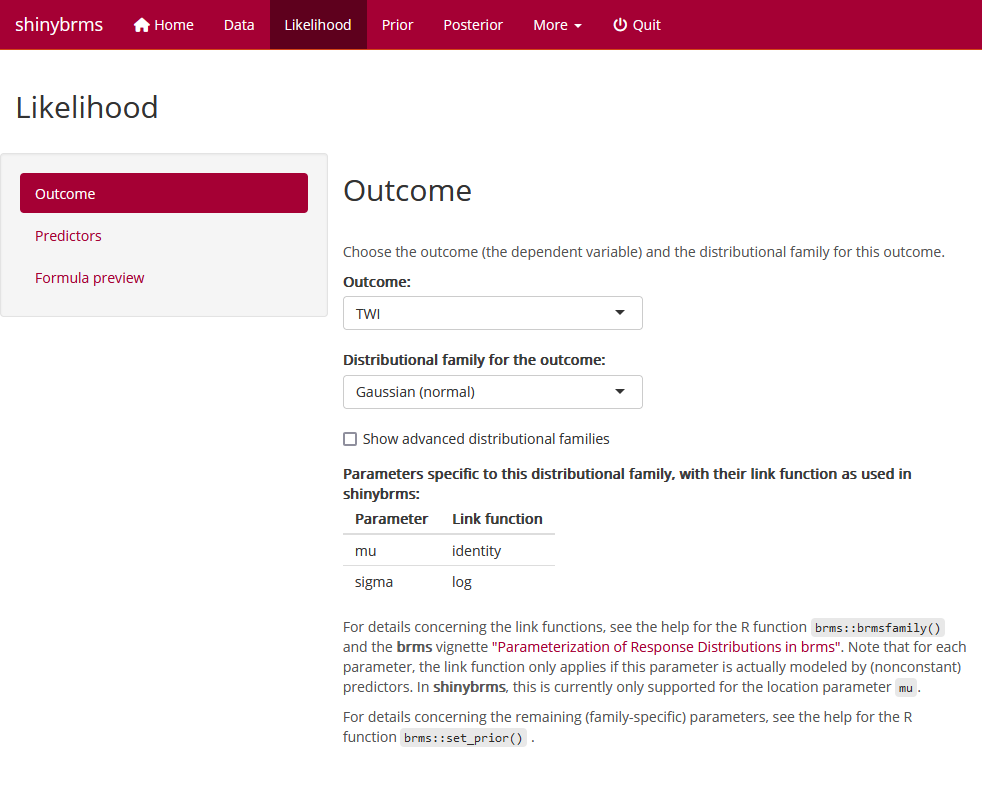
\includegraphics[width=\textwidth]{Figures/Likelihood_Outcome.png}
  \caption[Tab ``Outcome'']{Tab ``Outcome'' on page ``Likelihood''.
  In the example presented here, we select~\code{TWI} as the outcome variable and the
  Gaussian family as the distributional family for this outcome.
  Tab ``Outcome'' and tab ``Predictors'' (Figure~\ref{fig:predictors}) are the two
  main components of page ``Likelihood''.}
  \label{fig:outcome}
\end{figure}%

On tab ``Predictors'' (Figure~\ref{fig:predictors}), we choose
\code{age}, \code{anticoagulation}, \code{diabetes}, \code{day}, and
\code{trt} to have population-level main effects and \code{patID} to have group-level
main effects (``random intercepts''). Further down on tab
``Predictors'', we add an interaction between \code{day} and \code{trt}
(not shown here). This interaction is included because the
TWI is supposed to show a stronger time-dependence in the two wound areas than
in the healthy skin area. Additionally, the TWI difference (in means) between
the standard and the CAP treatment might change over time.
\begin{figure}[t!]
  \centering
  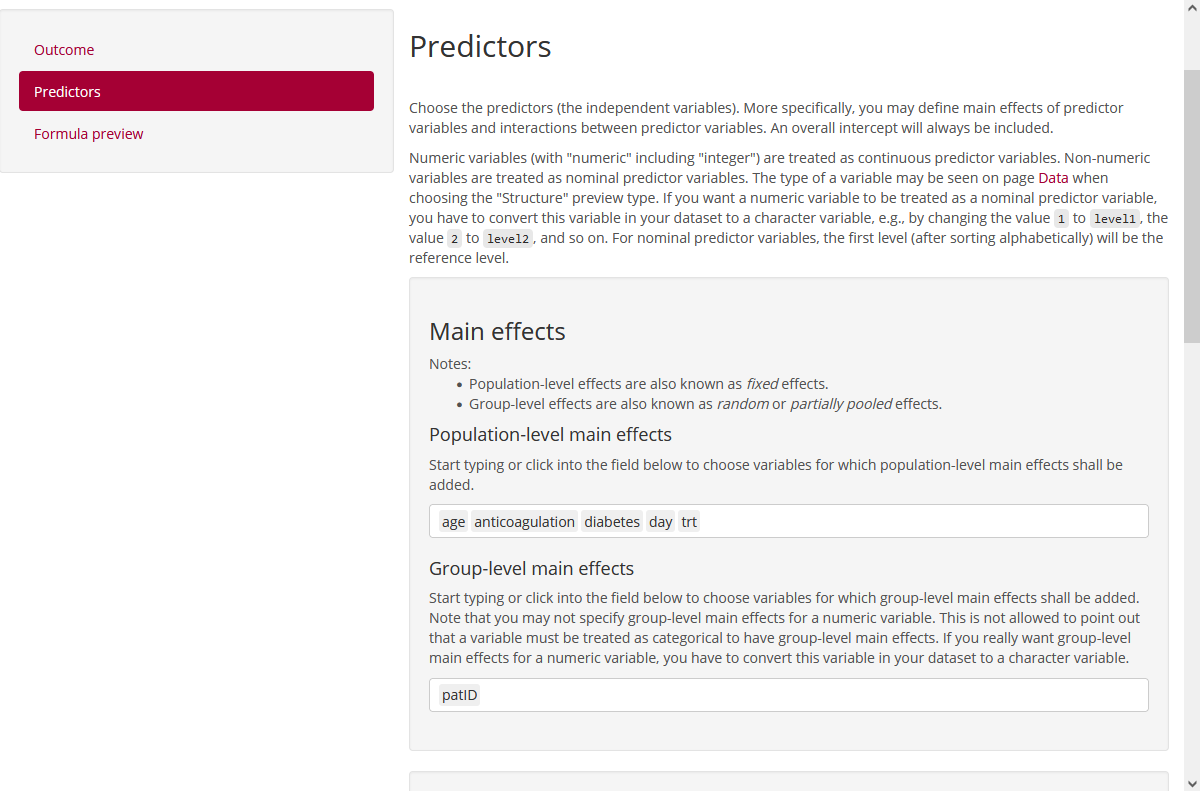
\includegraphics[width=\textwidth]{Figures/Likelihood_Predictors.png}
  \caption[Tab ``Predictors'']{Tab ``Predictors'' on page ``Likelihood''.
  Here, the main effects of the predictors need to be defined first (in the example presented here:
  variables \code{age}, \code{anticoagulation}, \code{diabetes}, \code{day}, \code{trt}, and \code{patID}).
  Then, further down on this tab (not visible here), interactions can be specified (in the
  example presented here: an interaction between variables \code{day} and \code{trt}).
  In principle, offsets may also be specified further down on this tab (not visible here),
  but our example does not feature offsets. For the main effects, the user may choose between
  population-level and group-level effects. For interaction effects, this choice will be performed 
  automatically based on the involved main effects.}
  \label{fig:predictors}
\end{figure}%

Now the likelihood is set up, so we can proceed with the prior. The default
priors (Figure~\ref{fig:prior-def}) are reasonable, but suppose we wanted a
weakly informative Student-$t$ prior with $3$~degrees of freedom, a location
parameter of~$0$, and a scale parameter of~$30$ for all regression
coefficients. To add this custom prior, we choose parameter class \code{b}
from the corresponding drop-down list shown in Figure~\ref{fig:prior-cust},
enter \code{student\_t(3,~0,~30)} into the input field entitled ``Prior
distribution'', and click the ``Add prior'' button. After doing so, our
Student-$t$ prior is added to the preview table (Figure~\ref{fig:prior-cust},
right-hand side). For all remaining parameters for which we do not specify a
custom prior, the corresponding default prior will be used.
\begin{figure}[t!]
  \centering
  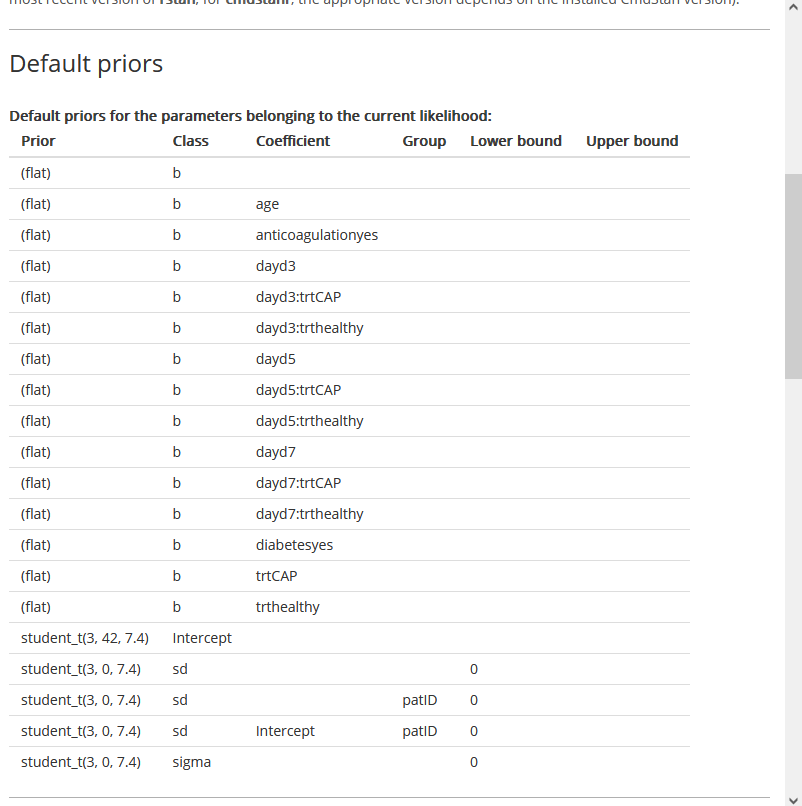
\includegraphics[width=0.7\textwidth]{Figures/Prior_Default.png}
  \caption[Section ``Default priors'']{Section ``Default priors'' on page ``Prior''.
  The default priors are taken from \pkg{brms} and depend on the currently specified
  likelihood. They can be overridden by custom priors (Figure~\ref{fig:prior-cust}).}
  \label{fig:prior-def}
\end{figure}%
\begin{figure}[t!]
  \centering
  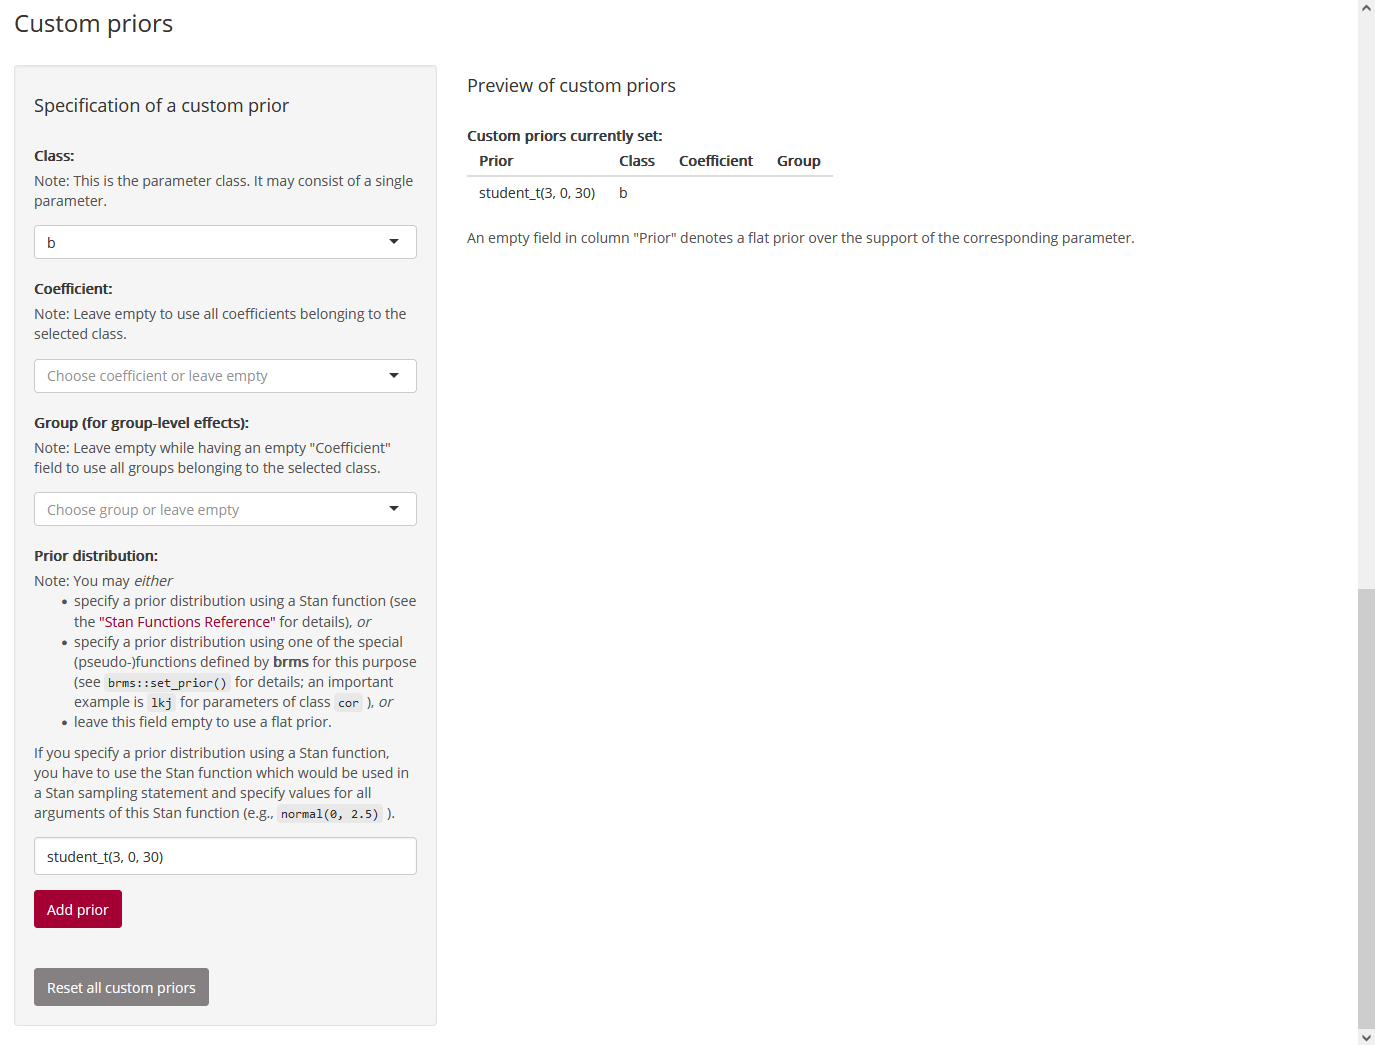
\includegraphics[width=\textwidth]{Figures/Prior_Custom.png}
  \caption[Section ``Custom priors'']{Section ``Custom priors'' on page ``Prior''.
  Here, we specify a Student-$t$ prior with $3$~degrees of freedom, a location
  parameter of~$0$, and a scale parameter of~$30$ for all regression
  coefficients (parameter class \code{b}). This overrides the default flat prior
  for these parameters (Figure~\ref{fig:prior-def}).}
  \label{fig:prior-cust}
\end{figure}%

Now the model is fully set up, so we can start inferring the posterior. To do
this, we switch to page ``Posterior'' where
we scroll down to the advanced options on tab ``Run Stan''
(Figure~\ref{fig:post-run-advOpts}). There, we set a seed for reproducibility.
Afterwards, we scroll further down to panel ``Run Stan'' where we
click the button for starting the Stan run
(Figure~\ref{fig:post-run-run}). For this example, the Stan run as a
whole (including the compilation of the C++ code) takes about 50 seconds
on a standard desktop machine.
\begin{figure}[t!]
  \centering
  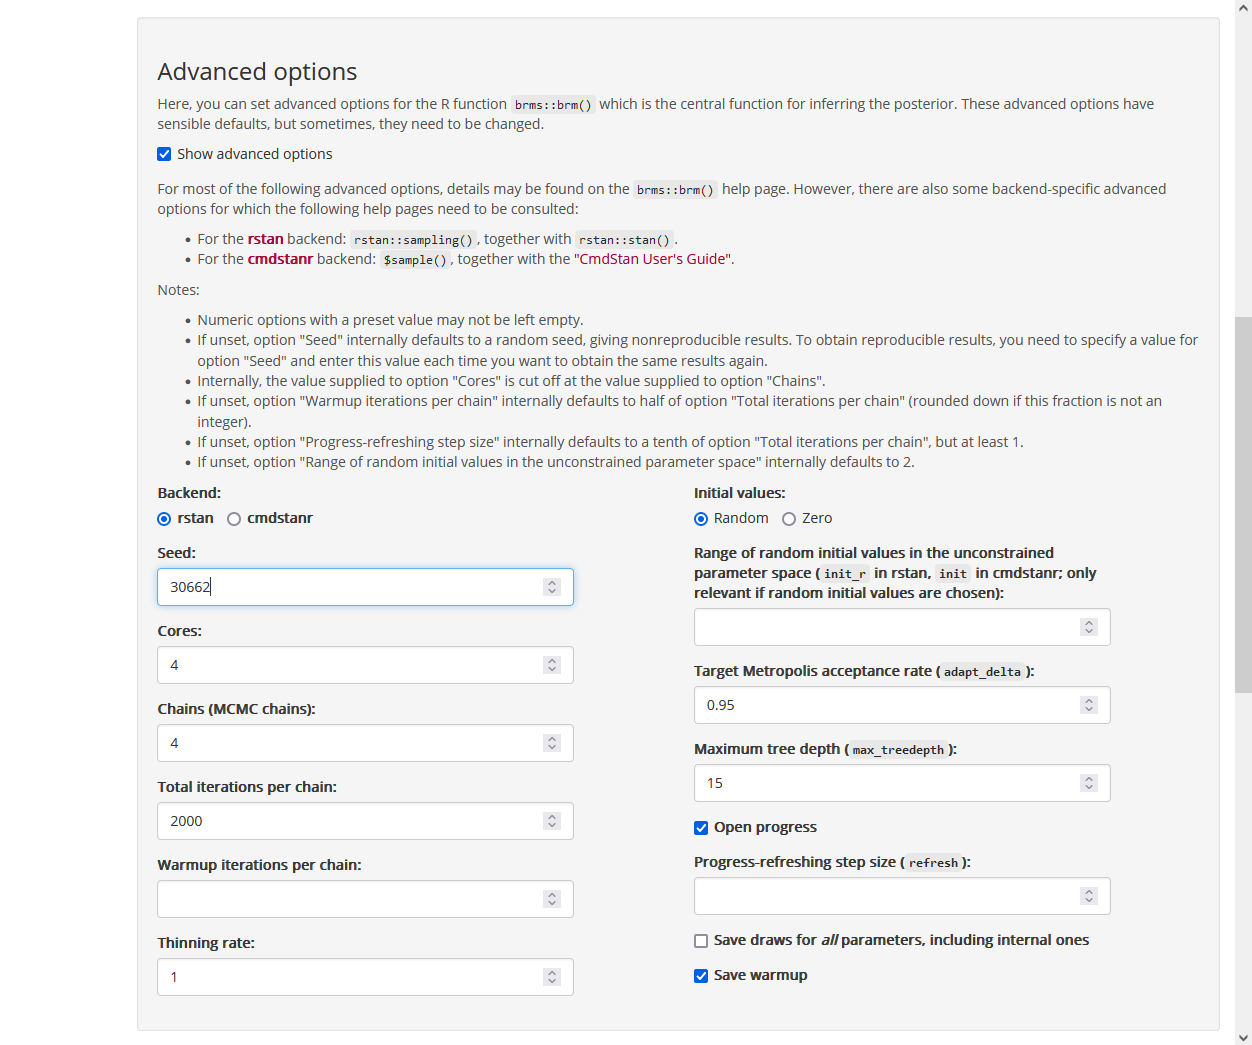
\includegraphics[width=\textwidth]{Figures/Posterior_Run_AdvOpts.png}
  \caption[Panel ``Advanced options'']{Panel ``Advanced options'' on
  tab ``Run Stan'' of page ``Posterior''.
  The defaults for these advanced options should be fine for most practical
  situations. In the example presented here, we only set a specific seed so
  that results are reproducible.}
  \label{fig:post-run-advOpts}
\end{figure}%
\begin{figure}[t!]
  \centering
  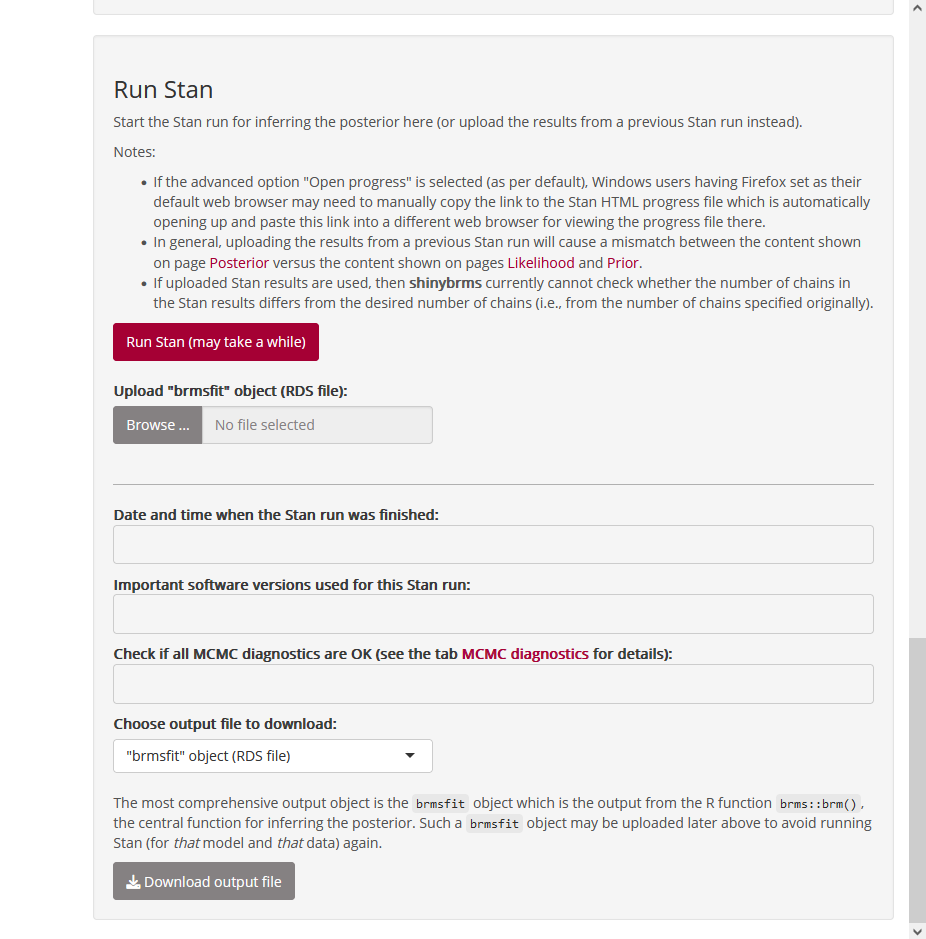
\includegraphics[width=\textwidth]{Figures/Posterior_Run_Run.png}
  \caption[Panel ``Run Stan'']{Panel ``Run Stan'' on tab ``Run Stan'' of page ``Posterior''.
  This is the central UI element: By clicking the red button, the Stan run
  is started, which first involves several preparation steps (including the
  compilation of the C++ code) and then the MCMC sampling itself.}
  \label{fig:post-run-run}
\end{figure}%

After Stan has finished sampling, we receive a pop-up notification (not
shown here) whether all MCMC diagnostics have passed their checks. Here, this
is the case as we may also see on tab ``MCMC diagnostics''
(Figure~\ref{fig:post-MCMC}).
\begin{figure}[t!]
  \centering
  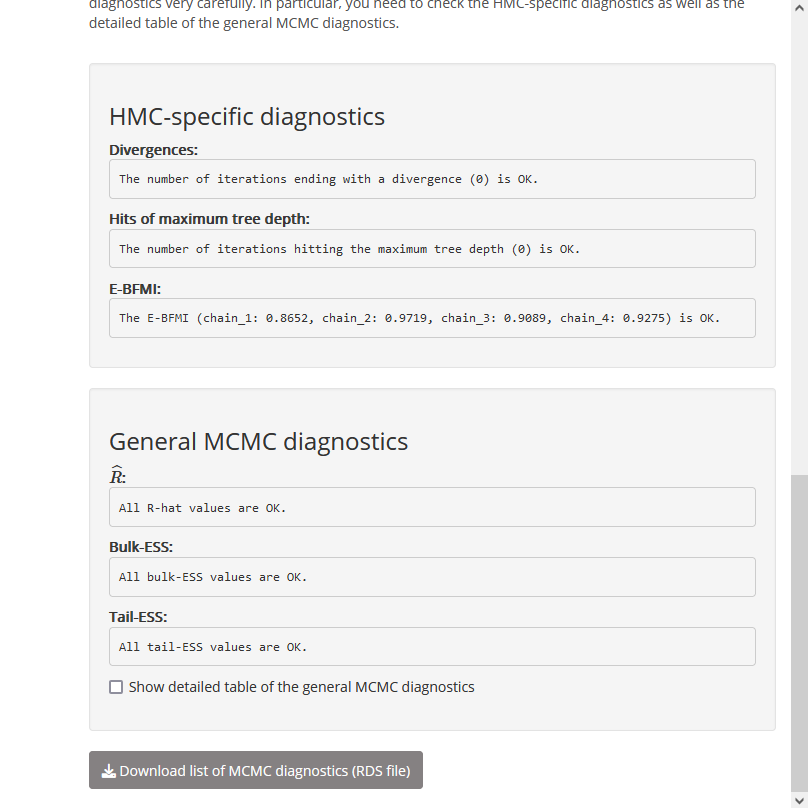
\includegraphics[width=\textwidth]{Figures/Posterior_Diagnostics.png}
  \caption[Tab ``MCMC diagnostics'']{Tab ``MCMC diagnostics'' on page ``Posterior''.
  This tab presents the diagnostics from section~\nameref{tab-MCMC}, applied to
  the user's Stan run (for the exact values of the general MCMC diagnostics, the
  checkbox ``Show detailed table of the general MCMC diagnostics'' needs to be
  checked). The purpose of this tab is to obtain details about problematic
  MCMC diagnostics in case there are such (after the Stan run, the user always
  receives a notification stating if there are problematic MCMC diagnostics or not).}
  \label{fig:post-MCMC}
\end{figure}%

Since \pkg{shinybrms} reports all MCMC diagnostics as being OK, we may start
interpreting the posterior. On tab ``Default summary''
(Figure~\ref{fig:post-smmry}), it is mainly the summary of the population-level
effects which is of interest here: With each additional year of \code{age}, the
TWI is estimated to increase by ca. $0.10$ with a $95\,\%$ CrI of ca.
$(-0.28, 0.48)$. An \code{anticoagulation} therapy is estimated
to increase the TWI by ca. $-1.12$ with a $95\,\%$ CrI of ca.
$(-7.53, 5.69)$. A \code{diabetes} disease is estimated to increase the TWI by
ca. $-0.56$ with a $95\,\%$ CrI of ca. $(-6.51, 5.66)$. As may be
seen from these three CrIs, the statistical uncertainty is
quite big which is probably due to the small~$P = 10$.
\begin{figure}[t!]
  \centering
  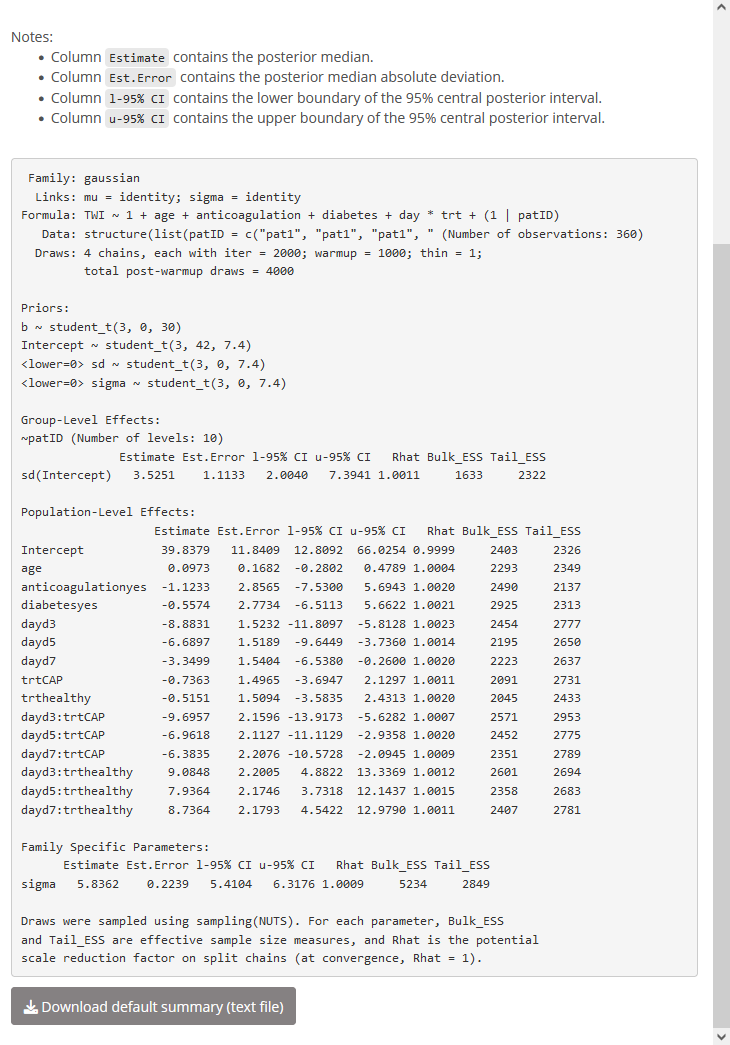
\includegraphics[width=\textwidth]{Figures/Posterior_Summary.png}
  \caption[Tab ``Default summary'']{Tab ``Default summary'' on page ``Posterior''.
  Presented is the output of method \code{brms:::summary.brmsfit()} with arguments
  \code{priors} and \code{robust} set to \code{TRUE} (causing the priors to be
  shown, too, and the more robust summary quantities median and
  median absolute deviation to be used instead of the less robust quantities
  mean and standard deviation).
  This tab is only intended for a quick inspection (the \pkg{shinystan} app
  offers a more comprehensive output).}
  \label{fig:post-smmry}
\end{figure}%

Since we included an interaction between \code{day} and \code{trt}, the
coefficients for these two variables are most conveniently interpreted by the
help of a custom summary (Figure~\ref{fig:post-custsmmry}) and a
conditional-effects plot (Figure~\ref{fig:post-ceff}). On tab ``Custom
summary'' (Figure~\ref{fig:post-custsmmry}), we may calculate the estimated TWI
difference (in means) between the CAP and the standard treatment separately
for each \code{day} by entering the corresponding sum expressions (and the
expression \code{`b\_trtCAP`} for day 1) in turn. The resulting table is included
in Figure~\ref{fig:post-custsmmry}: On day 1 (where the two wound areas had not
been treated yet), the standard treatment and the CAP treatment lead to a
quite similar TWI (the posterior median of their TWI difference being ca.
$-0.74$ with a $95\,\%$ CrI of ca. $(-3.69, 2.13)$). In
contrast, on days 3, 5, and 7, the CAP treatment clearly leads to a
\emph{lower} TWI than the standard treatment (posterior medians of ca.
$-10.45$, $-7.66$, and $-7.10$, respectively, and $95\,\%$ CrIs
of ca. $(-13.43, -7.36)$, $(-10.63, -4.84)$, and $(-10.11, -4.03)$,
respectively). This answers the primary research question: The CAP treatment
indeed leads to a decreased TWI and therefore an improved wound healing
compared to the standard treatment. This is also well illustrated by the
conditional-effects plot (Figure~\ref{fig:post-ceff}). The conditional-effects
plot also confirms that the TWI in the healthy skin area does not change as
heavily over time as in the two wound areas.
\begin{figure}[t!]
  \centering
  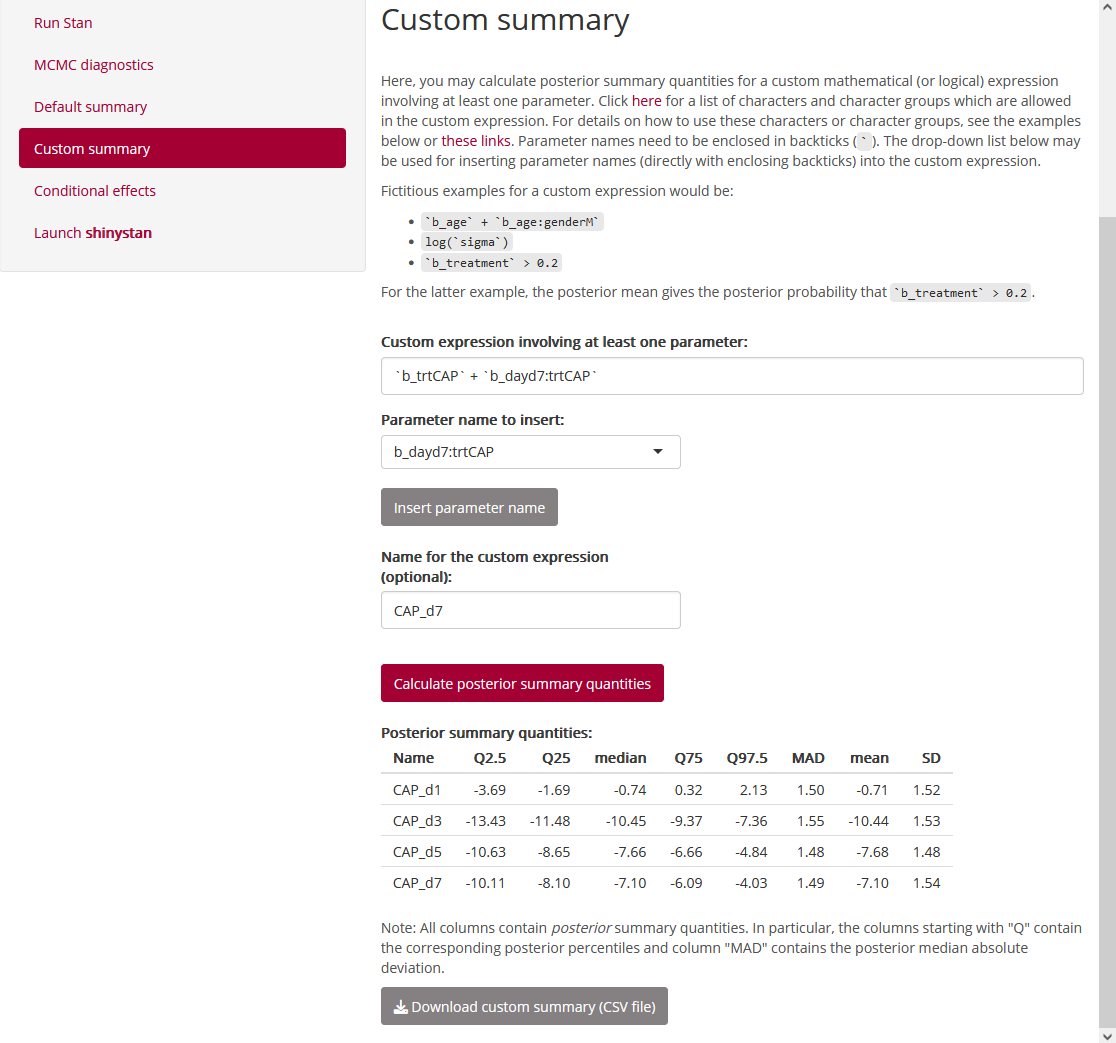
\includegraphics[width=\textwidth]{Figures/Posterior_CustSummary.png}
  \caption[Tab ``Custom summary'']{Tab ``Custom summary'' on page ``Posterior''.
  In contrast to tab ``Default summary'' (Figure~\ref{fig:post-smmry}), users
  can request their own summary quantities here. In the example presented here,
  we calculate the \code{day}-specific \code{CAP} effects. These show that apart
  from day 1 (where the wound areas had not been treated yet), the CAP treatment
  leads to a lower (i.e., better) TWI compared to the standard treatment (which
  is the reference category), with the posterior median ranging from
  ca.~$-10.45$ to ca.~$-7.10$ on days 3, 5, and 7.}
  \label{fig:post-custsmmry}
\end{figure}%
\begin{figure}[t!]
  \centering
  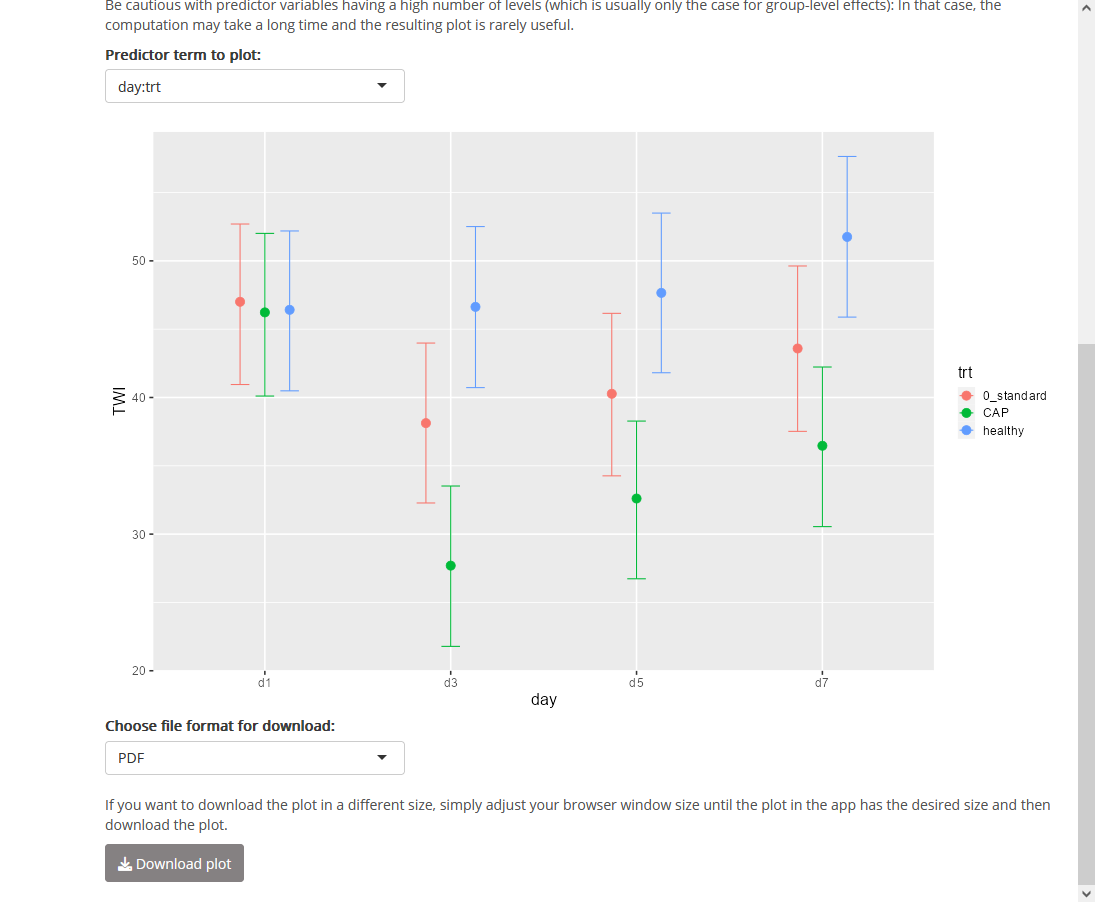
\includegraphics[width=\textwidth]{Figures/Posterior_CondEff.png}
  \caption[Tab ``Conditional effects'']{Tab ``Conditional effects'' on page ``Posterior''.
  This tab shows the conditional-effects plots produced by \code{brms::conditional\_effects()}.
  In the example presented here, we select the conditional-effects plot for the
  \code{day:trt} interaction. Similarly to Figure~\ref{fig:post-custsmmry}, this demonstrates
  that apart from day 1, the CAP treatment leads to a lower TWI compared to the standard
  treatment. This plot also illustrates that in the healthy skin area, the TWI is roughly
  constant over time, with a slight increase on day 7.}
  \label{fig:post-ceff}
\end{figure}%

Finally, we switch to tab ``Launch \pkg{shinystan}'', enter a seed for
the reproducibility of the PPCs (here, \code{63438}), and click on the button
for launching \pkg{shinystan}.

%%%%%%%%%%%%%%%%%%
\subsection[shinystan]{\pkg{shinystan}}
\label{exmpl-shinystan}

Within \pkg{shinystan}, we may inspect some PPC plots, e.g., a kernel density
estimate for the observed TWI values, overlaid by kernel density estimates for
replicated TWI values (Figure~\ref{fig:shinystan-ppc-overlay}). This overlaid
density plot suggests that the model is appropriate, being able to generate
outcome values similar to the observed ones after having estimated the unknown
parameters by the help of the observed dataset (as well as the prior).
Nevertheless, the model may still be improved, as illustrated by
the PPC plots shown in Figure~\ref{fig:shinystan-ppc-stat} (lower two
histograms): The minimum of the observed TWI values is systematically smaller
than the replicated minimums, the opposite holding---even if not that
extremely---for the maximum. However, we consider the current model to be
appropriate for the primary research question.

With respect to the parameter estimates, \pkg{shinystan} offers, e.g., a
visualization of the posterior medians, together with $50\,\%$ and $95\,\%$
CrIs (Figure~\ref{fig:shinystan-intvls}). The \pkg{shinystan}
app also offers kernel density estimates for the univariate marginal
posteriors (not shown).
\begin{figure}[t!]
  \centering
  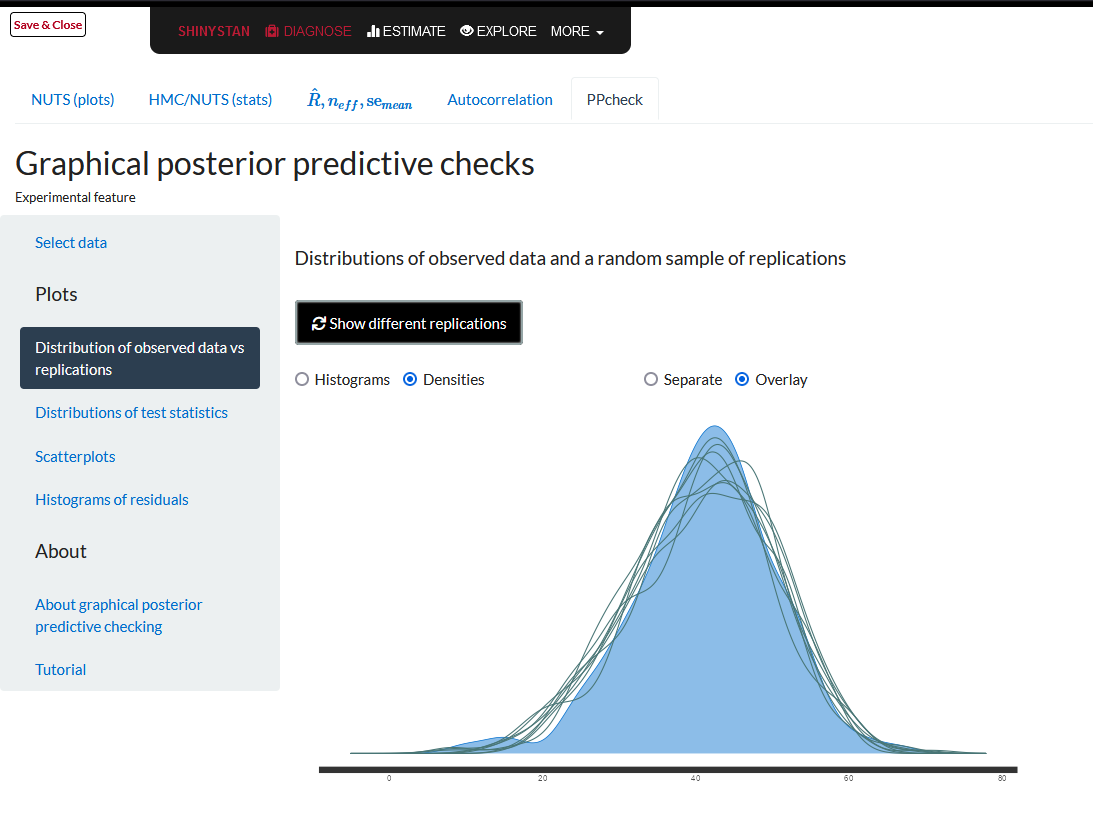
\includegraphics[width=\textwidth]{Figures/shinystan_PPC_overlay.png}
  \caption[\pkg{shinystan}: PPC (densities)]{\pkg{shinystan}: PPC \textit{via}
  overlaid kernel density estimates. The shaded blue density corresponds to the
  observed outcome values whereas each of the 8 overlaid green density lines
  corresponds to one randomly chosen post-warmup MCMC iteration.
  Here, the distributions of the model's predictions (which are based on the
  posterior, i.e., on the joint parameter distribution inferred from the data
  and the prior) are similar to the distribution of the observed outcome values,
  showing that at least in this regard, the model is a reasonable one.}
  \label{fig:shinystan-ppc-overlay}
\end{figure}%
\begin{figure}[t!]
  \centering
  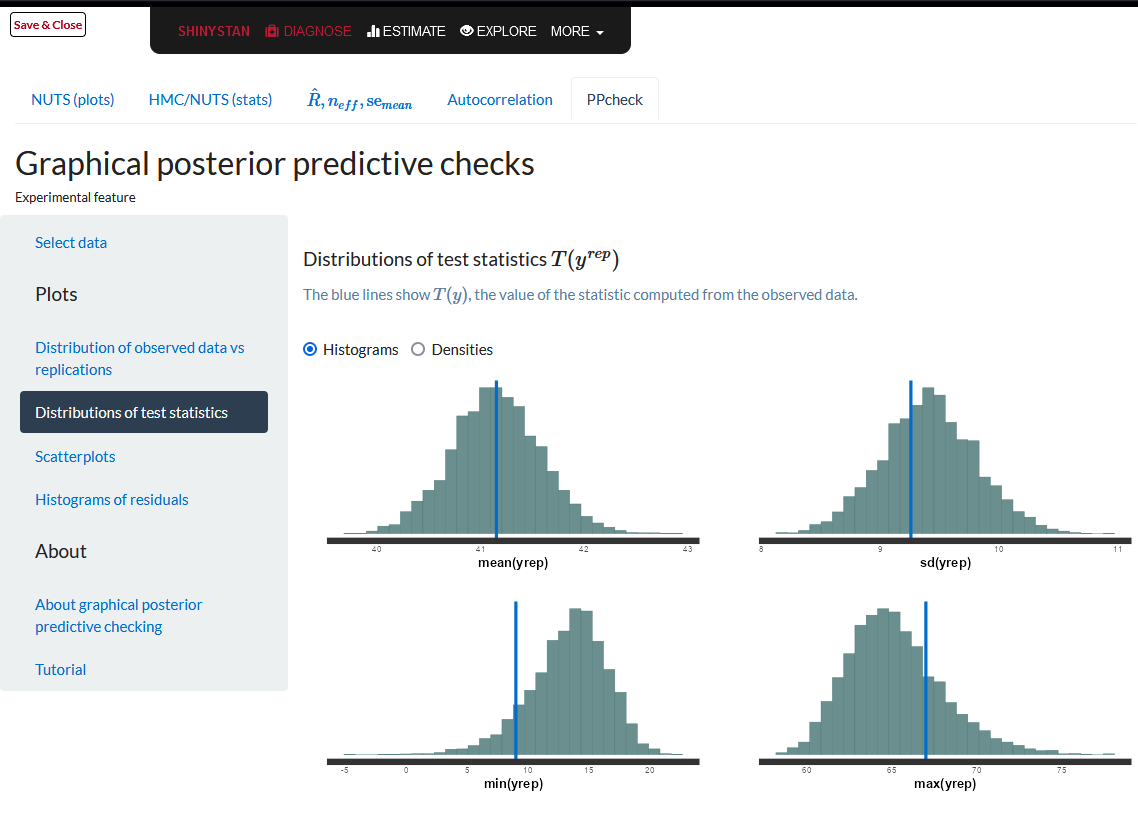
\includegraphics[width=\textwidth]{Figures/shinystan_PPC_stats.png}
  \caption[\pkg{shinystan}: PPCs (statistics)]{\pkg{shinystan}: PPCs \textit{via}
  summary statistics.
  In contrast to the PPC from Figure~\ref{fig:shinystan-ppc-overlay}, these PPCs here
  are based on \emph{all} posterior draws which is possible by aggregating across the
  observations. The aggregation statistics are the mean (top left), the standard
  deviation (top right), the minimum (bottom left), and the maximum (bottom right).
  Here, these aggregated predictions show some room for model improvement: The minimum
  is overestimated---or rather ``overpredicted''---by the model, the maximum is
  underestimated. Thus, the range of the replicated outcome values is narrower than
  the observed one. In contrast, the mean TWI is replicated reliably. The standard
  deviation shows a slight overestimation by the model. In summary, the Gaussian
  family seems to be a suboptimal outcome family, but we consider it to be sufficient
  for answering the primary research question (the comparison of CAP and standard
  treatment in terms of the central tendency of TWI values).}
  \label{fig:shinystan-ppc-stat}
\end{figure}%
\begin{figure}[t!]
  \centering
  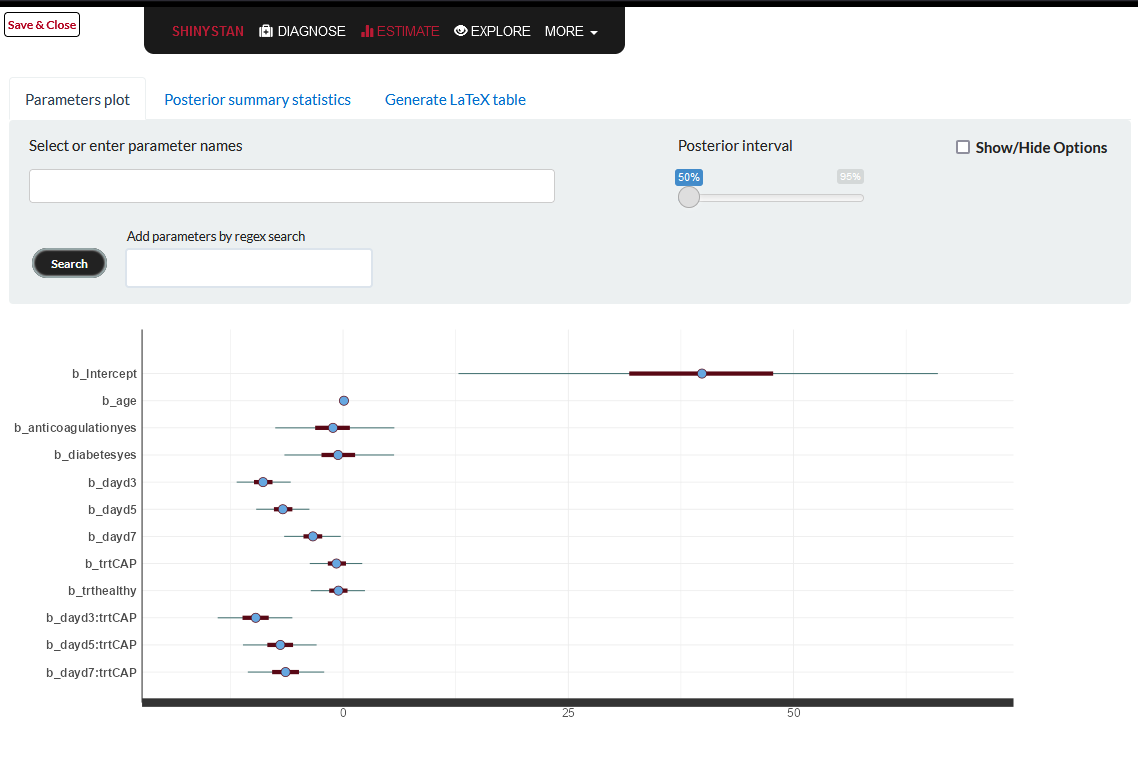
\includegraphics[width=\textwidth]{Figures/shinystan_intervals.png}
  \caption[\pkg{shinystan}: CrIs]{\pkg{shinystan}: Posterior intervals (credible
  intervals, CrIs). The default plot shown here is restricted to the first 12
  parameters. More parameters may be selected in the two input fields above the
  plot.
  The different scales of the parameters (in particular, the intercept and the
  regression coefficient for \code{age} are on strikingly different scales)
  illustrate that in interactive use, it often makes sense to customize the
  selection of parameters.}
  \label{fig:shinystan-intvls}
\end{figure}%

%%%%%%%%%%%%%%%%%%%%%%%%%%%%%%%%%%%%
\section{Discussion}
\label{disc}

We have presented our \pkg{shiny} app called \pkg{shinybrms}, distributed as
an R package. With the \pkg{shinybrms} GUI, we hope to make Bayesian
regression modeling more accessible for people without any knowledge of
R's syntax. Currently, the user still needs to execute some R code
for setting up \pkg{shinybrms}'s backend and for launching the \pkg{shinybrms}
app, even if he or she is using a GUI for installing R packages. We tried
to make this as easy as possible by providing step-by-step instructions in the
\file{README} file of the \pkg{shinybrms} package. More importantly
however, the \pkg{shinybrms} app may be hosted on a server and accessed through a
web browser, just like any other \pkg{shiny} app. In that case, the user does
not need to install the \pkg{shinybrms} package or any other additional
software. With the server-sided hosting, the \pkg{shinybrms} app may even be
accessed from a mobile device where it is usually impossible to install any
software designed for personal computers. Of course, setting up the
server-sided hosting is a lot more complex than following the instructions
from our \file{README} file for running \pkg{shinybrms} on a local
computer, but the idea is that IT departments of bigger institutions
could establish the server-sided hosting (potentially adding an access
control on top) and then members of that institution could access the
\pkg{shinybrms} app through their web browsers.

Note that JASP offers an alternative host-client service by relying on
rollApp \citep{rollapp_inc_rollapp_2020, rollapp_inc_jasp_2020}.

Apart from application in practice, \pkg{shinybrms} may also be valuable for
teaching Bayesian regression models, e.g., to undergraduate students.

Of course, \pkg{shinybrms} may still be extended. As may be seen from our
real-world example in section~\nameref{exmpl}, truncated outcome families would be
a useful feature. Apart from this, our future plans also include further
outcome families supported by \pkg{brms} (e.g., ordinal and time-to-event
regression), model selection features (e.g., using the package \CRANpkg{projpred}
by \citealp{piironen_projpred_2020}), and support for special \pkg{brms}
features such as smoothed effects and known measurement error in the outcome
variable (needed for meta-analyses). When implementing new features, the
challenge will be to keep the GUI as simple as possible: In our opinion, a GUI
such as \pkg{shinybrms} should support the user by automizing steps wherever
this is appropriate and thus focus the attention to steps which may not be
automized (in particular those related to the original research question).

\section{Supplementary Material}

This article comes with an online Supplement which consists of the following files:
\begin{itemize}
  \item file \file{Supplement\_sections.pdf} which is a document with the
  following sections:
  \begin{itemize}
    \item ``Existing GUIs'',
    \item ``Advanced distributional families'',
    \item ``Frequentist analysis of the example'';
  \end{itemize}
  \item file \file{CAP.csv} which contains the dataset for section~\nameref{exmpl};
  \item file \file{weber\_shinybrms.R} which contains the R code for section~\nameref{exmpl};
  \item file \file{weber\_shinybrms\_sessionInfo.txt} which contains the original
  computing environment information for section~\nameref{exmpl}. Note that the
  reproducibility of Stan results depends on the machine's hardware, so in general,
  our results from section~\nameref{exmpl} will not be perfectly reproducible on
  other machines.
\end{itemize}

\clearpage

\bibliography{weber_shinybrms}

\address{Frank Weber\\
  Institute for Biostatistics and Informatics in Medicine and Ageing Research\\
  Rostock University Medical Center\\
  Ernst-Heydemann-Str.~8\\
  18057 Rostock\\
  Germany\\
  ORCiD: \href{https://orcid.org/0000-0002-4842-7922}{0000-0002-4842-7922}\\
  \email{frank.weber@uni-rostock.de}}

\address{Katja Ickstadt\\
  Department of Statistics\\
  TU Dortmund University\\
  Vogelpothsweg 87\\
  44227 Dortmund\\
  Germany\\
  ORCiD: \href{https://orcid.org/0000-0001-5157-2496}{0000-0001-5157-2496}\\
  \email{ickstadt@statistik.tu-dortmund.de}}

\address{\"Anne Glass\\
  Institute for Biostatistics and Informatics in Medicine and Ageing Research\\
  Rostock University Medical Center\\
  Ernst-Heydemann-Str.~8\\
  18057 Rostock\\
  Germany\\
  ORCiD: \href{https://orcid.org/0000-0002-7715-9058}{0000-0002-7715-9058}\\
  \email{aenne.glass@uni-rostock.de}}
